\cite{chabinUsingGraphGrammar2019} s'appuie sur la réécriture de graphes pour la maintenance des graphes \gls{rdf}.
Étant donné une base \gls{rdf} modélisée avec le schéma \gls{rdfs}, l'objectif est de maintenir le respect des contraintes d'intégrité de \gls{rdfs} tel qu'expliqué dans \cite{flourisFormalFoundationsRDF2013}, \cite{halfeld-ferrariRDFUpdatesConstraints2017} ou encore \cite{chabinConsistentUpdatingDatabases2020} après mise à jour de l'instance.

Les règles de la sémantique \gls{rdfs} ont été ensuite exprimées sous forme de règles logique en utilisant les symboles de prédicats définis plus haut.
Si l'on prend la règle $\forall x,y~CI(x,y) \implies Cl(y)$, elle signifie que pour que tout $x$ soit instance de $y$ il faut que $y$ soit une classe.
Dans les travaux en cours au \gls{lifo}, l'idée est de proposer une vérification similaire, mais en utilisant les techniques de réécriture de graphes.
Dans ce cadre, les règles de la sémantique \gls{rdf} sont décrites via des règles de réécriture de graphe.

L'exemple figure~\ref{fig:gram_rule} illustre comment les règles de la sémantique \gls{rdf} sont modélisées dans le cadre de la réécriture de graphes.

\begin{figure}[ht]
    \centering
    \begin{subfigure}[b]{.3\textwidth}
        \centering
        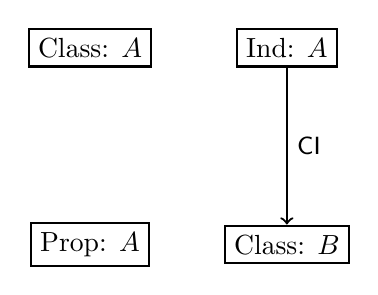
\begin{tikzpicture}[->,auto,node distance=2.5cm,thick,main node/.style={draw}]
            \node[main node] (1) {Class: $A$};
            \node[main node] (2) [below of=1] {Prop: $A$};
            \node[main node] (3) [right of=1] {Ind: $A$};
            \node[main node] (4) [right of=2] {Class: $B$};
            \path[every node/.style={font=\sffamily\small}]
            (3) edge node {CI} (4);
        \end{tikzpicture}
        \caption{NAC}
        \label{fig:gram_rule:nac}
    \end{subfigure}
    \begin{subfigure}[b]{.3\textwidth}
        \centering
        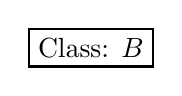
\begin{tikzpicture}[->,auto,node distance=2.5cm,thick,main node/.style={draw}]
            \node[main node] (2) {Class: $B$};
        \end{tikzpicture}
        \caption{LHS}
        \label{fig:gram_rule:lhs}
    \end{subfigure}
    \begin{subfigure}[b]{.3\textwidth}
        \centering
        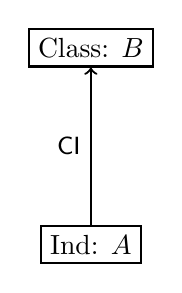
\begin{tikzpicture}[->,auto,node distance=2.5cm,thick,main node/.style={draw}]
            \node[main node] (1) {Class: $B$};
            \node[main node] (2) [below of=1] {Ind: $A$};
            \path[every node/.style={font=\sffamily\small}]
            (2) edge node {CI} (1);
        \end{tikzpicture}
        \caption{RHS}
        \label{fig:gram_rule:rhs}
    \end{subfigure}
    \caption{Règle de réécriture simplifiée pour le fait $CI(A,B)$}
    \label{fig:gram_rule}
\end{figure}

\paragraph{}
Une grammaire est un ensemble de règles définissant un langage.
Ces règles de réécritures sont des fonctions qui, pour une entrée donnée donne une nouvelle sortie.
Les grammaires permettent de définir l'ensemble des "mots" valide pour un langage donné.
Les grammaires de graphes sont des grammaires appliquées aux graphes.
Les règles de réécriture de graphes sont de la forme $\text{LHS} \implies \text{RHS}$ où \gls{lhs} est un motif et \gls{rhs} le résultat de l'application de la règle.
Il existe un morphisme entre \gls{lhs} et \gls{rhs} définissant comment la règle doit être appliquée (dans l'exemple précédent, un morphisme existe sur la classe $B$).
Une règle est applicable s'il existe un isomorphisme entre \gls{lhs} et le graphe $G$ que l'on construit.
Il est possible d'ajouter des \gls{nac}, comme \gls{lhs} elles permettent de définir un pattern qui, s'il trouve un isomorphisme dans $G$, rend la règle inapplicable (Dans l'exemple, les \gls{nac}s sont utilisées pour éviter l'insertion du fait s'il est déjà présent dans la base ou si le type de $A$ n'est pas le bon).

Les règles ne peuvent s'appliquer que si leur application maintient la cohérence.
Nous allons plus loin et proposons avec \gls{setup} de donner la priorité aux mises à jour.
Nous définissons un ensemble d'effet de bords qui doivent être réalisés pour modifier la base afin de rendre les règles applicables et de prioriser l'ajout d'un fait.
Ces effets de bords se basent sur la sémantique de \gls{rdfs} et la cohérence de la base est garantie pendant la modification, car cette dernière ne fait qu'appeler des règles de réécriture respectant elle-même la cohérence de la base.

Considérons une base de connaissance cohérente représentée par le graphe $G$ figure~\ref{fig:rule_ci}.
Si l'on veut appliquer la règle de réécriture figure~\ref{fig:gram_rule} on remarque que la règle ne peut pas s'appliquer, car la \gls{nac} est vérifiée ($A$ est une classe).
Il faut donc appliquer un effet de bords pour supprimer ce fait (en rouge).
La règle devient alors applicable (en bleu).

\begin{figure}
    \centering
    \begin{subfigure}[b]{.45\textwidth}
        \centering
        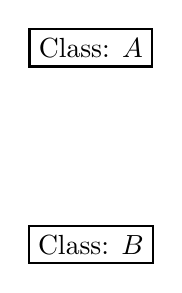
\begin{tikzpicture}[->,auto,node distance=2.5cm,thick,main node/.style={draw}]
            \node[main node] (1) {Class: $A$};
            \node[main node] (2) [below of=1] {Class: $B$};
        \end{tikzpicture}
    \end{subfigure}
    \raisebox{1.5cm}{\scalebox{1.5}{$\longrightarrow$}}
    \begin{subfigure}[b]{.45\textwidth}
        \centering
        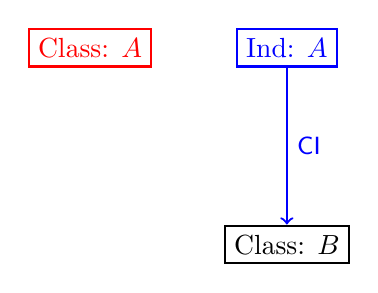
\begin{tikzpicture}[->,auto,node distance=2.5cm,thick,main node/.style={draw}]
            \node[main node] (1) [color=red] {Class: $A$};
            \node[main node] (2) [right of=1, color=blue] {Ind: $A$};
            \node[main node] (3) [below of=2] {Class: $B$};
            \path[every node/.style={font=\sffamily\small}]
            (2) edge [color=blue] node {CI} (3);
        \end{tikzpicture}
    \end{subfigure}
    \caption{Application de la règle $CI(A,B)$}
    \label{fig:rule_ci}
\end{figure}

\paragraph{}
Bien que l'objectif premier est de donner la priorité à la mise à jour sur l'ensemble de la base, \cite{chabinUsingGraphGrammar2019} propose différents niveaux de modification autorisés.
Ce niveau peut être paramétré pour chaque utilisateur lui donnant ainsi certains droits de modification.
Le niveau le plus élevé est autorisé à modifier le schéma et l'instance pour ajouter un fait.
Un niveau moins élevé permet seulement de modifier l'instance tandis que le niveau le plus bas ne peut pas modifier la base et peut donc seulement ajouter ou supprimer un fait si la cohérence de la base est maintenue.

\begin{figure}
    \begin{eqnarray}
        Cl(x)\\
        Cl(y) \lor (y = Resource)\\
        \neg CSub(y, x)\\
        \forall~z CSub(y, z) \implies CSub(x, z)\\
        \forall~z CSub(z, x) \implies CSub(z, y)\\
        \forall~z_i CI(z_i, x) \implies CI(z_i, y) \label{eq:rule_csub:ci}
    \end{eqnarray}
    \caption{Effets de bord pour l'ajout du fait $CSub(x, y)$}
    \label{eq:rule_csub}
\end{figure}

\paragraph{}
La figure~\ref{fig:app_rule} représente une base de connaissance initiale (en noir) et les modifications nécessaires (en bleu) pour l'ajout du fait $CSub(C_1, C_2)$.
En suivant les effets de bords figure~\ref{eq:rule_csub}, l'ajout du fait $CSub(C_1, C_2))$ implique que $C_1$ et $C_2$ soient des classes.
Comme $C_2$ n'est pas présent, le schéma doit être modifié.
Le fait $CSub(C_2, Resource)$ est alors ajouté.
Par la suite, le fait $CSub(C_1, C_2))$ peut être ajouté en ajoutant aussi le fait $CI(I, C_2)$ par transitivité de la relation $CI$ (figure~\ref{eq:rule_csub}(\ref{eq:rule_csub:ci})).
Cet exemple montre l'application d'effets de bords pour rendre applicable une règle.
Sans ces effets de bords, il aurait été impossible d'ajouter le fait voulu tout en respectant les règles d'intégrités.
Ici, notre individu est bien l'instance d'une classe et de toutes les sous-classes associées.
La base avant et après application de la règle est un graphe \gls{rdfs} valide.

\begin{figure}[htb]
    \centering
    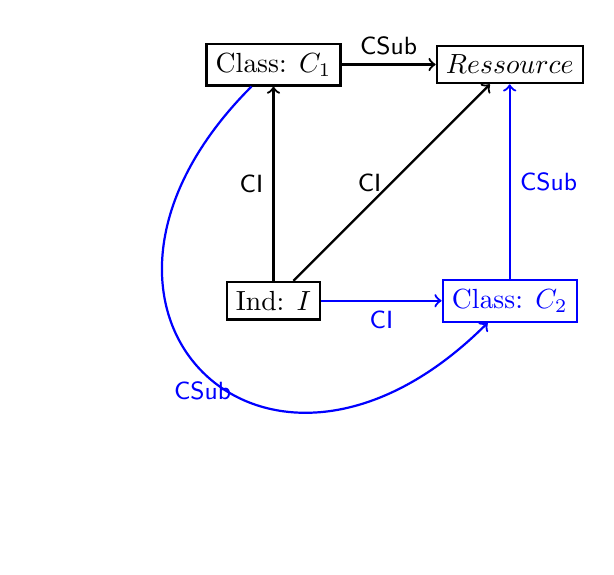
\begin{tikzpicture}[->,auto,node distance=3cm,thick,main node/.style={draw}]
        \node[main node] (1) {Ind: $I$};
        \node[main node] (2) [above of=1] {Class: $C_1$};
        \node[main node] (3) [right of=1, color=blue] {Class: $C_2$};
        \node[main node] (4) [above of=3] {$Ressource$};
        \path[every node/.style={font=\sffamily\small}]
        (1) edge node [left] {CI} (2)
        (1) edge [color=blue] node [below] {CI} (3)
        (1) edge node [left] {CI} (4)
        (2) edge node [above] {CSub} (4)
        (2) edge [color=blue, distance=4cm, bend right=90] node [below] {CSub} (3)
        (3) edge [color=blue] node [right] {CSub} (4);
    \end{tikzpicture}
    \caption{Exemple de modification pour l'application d'une règle}
    \label{fig:app_rule}
\end{figure}

\paragraph{}
Concrètement, l'ensemble des travaux de \gls{setup} constituent les bases pour la création automatique d'une base de connaissances dans notre projet.
Dans un premier temps, il est nécessaire de construire l'instance en suivant les règles de \gls{rdfs}.
\gls{pullup} fournirait un ensemble de faits qu'il suffit d'ajouter à notre base par l'intermédiaire de \gls{setup}, ce dernier à ici pour objectif de construire un schéma (classes et propriétés) qui respecte \gls{rdfs} à partir des données brutes extraites.

Bien que \gls{setup} autorise des mises à jour cohérentes dans une base de données graphe, il ne peut cependant pas être utilisé pour la construction d'une base complète.
L'application de règles de réécritures sur des graphes est d'une grande complexité (à cause de la détection d'isomorphisme).
Bien que cela soit suffisant pour une mise à jour dans une petite base, une modification impliquant de nombreux changements et application de règles est inutilisable en production.
De plus, l'implémentation actuelle n'a pas de fonctionnalité de type "fallback" permettant d'annuler les changements effectués sur la base en cas d'échec de la mise à jour.
Bien que l'on donne la priorité aux mises à jour, si l'on autorise seulement les modifications de l'instance, il est possible de ne pouvoir ajouter un fait.
